

\chapter{数值结果验证}

\section{基准算例}
\subsection{静态IAEA PWR三维基准问题}
\label{sec:result.test.iaea}

IAEA 三维压水堆基准题是三维两群扩散基准题\cite{center1977benchmark},
由177个燃料组件构成,堆芯取$1/4$,
大小为170cm $\times$ 170cm $\times$ 380cm,
堆芯的几何结构见\floatref{fig:result.test.iaea},
堆芯中心为对称边界条件,外侧边界入流为0,外侧也可取等效边界条件
\begin{align}
  \frac{\partial \phi_g}{\partial n}=-\frac{0.4692}{D_g}\phi_g
\end{align}

各材料界面见\floatref{tab:result.test.iaea.mat},
裂变谱取$\chi_1=1$,$\chi_2=0$。

\begin{table}
\centering
\caption{\label{tab:result.test.iaea.mat}静态IAEA PWR 三维基准题材料截面}
\begin{tabular}{cccccc}
\toprule
材料 & 能群$g$ & $D_g/\mathrm{cm}$ & $\Sigma_{a,g}/\mathrm{cm}^{-1}$
    & $\nu\Sigma_{f,g}/n,\mathrm{cm}^{-1}$
    & $\Sigma_{s,1\rightarrow2}/\mathrm{cm}^{-1}$\\
\midrule
\multirow{2}{*}{M1} 
  & 1 & 1.5 & 0.01 & 0 & \multirow{2}{*}{0.02} \\
  & 2 & 0.4 & 0.08 & 0.135 &\\
\multirow{2}{*}{M2} 
  & 1 & 1.5 & 0.01 & 0 & \multirow{2}{*}{0.02} \\
  & 2 & 0.4 & 0.085 & 0.135 &\\
\multirow{2}{*}{M3} 
  & 1 & 1.5 & 0.01 & 0 & \multirow{2}{*}{0.02} \\
  & 2 & 0.4 & 0.13 & 0.135 &\\
\multirow{2}{*}{M4} 
  & 1 & 2.0 & 0 & 0 & \multirow{2}{*}{0.04} \\
  & 2 & 0.3 & 0.01 & 0 &\\
\multirow{2}{*}{M5} 
  & 1 & 2.0 & 0 & 0 & \multirow{2}{*}{0.04} \\
  & 2 & 0.3 & 0.055 & 0 &\\
\bottomrule
\end{tabular}
\end{table}

\begin{figure}
\centering
\begin{subfigure}{\textwidth}
\centering
\begin{tikzpicture}[scale=0.7, transform shape]
\def\lenscale{0.06}

\def\x#1{#1*\lenscale}
\def\zz#1{#1*\lenscale-8}
\def\z#1{#1*\lenscale}

\draw [very thick] (0,0) -- (\x{170},0) 
            -- (\x{170}, \zz{380}) -- (0, \zz{380});
\draw [loosely dashdotted] (0,0) -- (0, \zz{380});
\draw (0,\z{20}) -- (\x{150},\z{20}) -- (\x{150},\zz{360}) -- (0,\zz{360});
\draw (\x{10},\z{20}) -- (\x{10},\zz{380});
\draw [dashed] (\x{30},\zz{380}) -- (\x{30},\zz{280}) -- (\x{50},\zz{280}) -- (\x{50},\zz{380});
\draw (\x{70},\z{20}) -- (\x{70},\zz{380});
\draw (\x{90}, \z{20}) -- (\x{90},\zz{380});
\draw (\x{130},\z{20}) -- (\x{130},\zz{360});
\node at (\x{10},\z{80}) {\huge $\approx$};
\node at (\x{70},\z{80}) {\huge $\approx$};
\node at (\x{90},\z{80}) {\huge $\approx$};
\node at (\x{130},\z{80}) {\huge $\approx$};
\node at (\x{150},\z{80}) {\huge $\approx$};
\node at (\x{170},\z{80}) {\huge $\approx$};

\node [left] at (0,0) {\Large 0};
\node [left] at (0,\z{20}) {\Large 20};
\node [left] at (0,\zz{280}) {\Large 280};
\node [left] at (0,\zz{360}) {\Large 360};
\node [left] at (0,\zz{380}) {\Large 380};

\foreach \xp in {0, 10,30,50,70,90,130,150,170}
{
\node [above] at (\x{\xp},\zz{380}) {\Large \xp};
}

\node at (\x{160}, \zz{260}) {\Large M4};
\node at (\x{140}, \zz{260}) {\Large M1};
\node at (\x{110}, \zz{260}) {\Large M2};
\node at (\x{80}, \zz{260}) {\Large M3};
\node at (\x{40}, \zz{260}) {\Large M2};

\draw [-latex new, arrow head=3mm] (-1,\zz{260}) -- (\x{5}, \zz{260});
\node [left] at (-1, \zz{260}) {\Large M3};

%\draw [-latex new, arrow head=3mm] (-1,\zz{320}) -- (\x{40}, \zz{320});
%\node [left] at (-1, \zz{320}) {\Large Mp3};
\node at (\x{40}, \zz{320}) {\Large M3};

\node at (\x{80}, \zz{370}) {\Large M5};
\node at (\x{60}, \zz{370}) {\Large M4};
\node at (\x{40}, \zz{370}) {\Large M5};
\node at (\x{20}, \zz{370}) {\Large M4};

\draw [-latex new, arrow head=3mm] (-1,\zz{370}) -- (\x{5}, \zz{370});
\node [left] at (-1, \zz{370}) {\Large M5};

\node [above] at (-0.5,\zz{380}+0.5) {\Large cm};
\node [above] at (\x{170}+1,\zz{380}) {\Large cm};
\end{tikzpicture}
\caption{纵截面图}
\end{subfigure}
\begin{subfigure}{\textwidth}
\centering
\begin{tikzpicture}[scale=0.7, transform shape]
\def\lenscale{0.06}
\def\x#1{#1*\lenscale}

\draw [loosely dashdotted] (\x{170},0) -- (0,0) -- (0,\x{170});
%\draw [loosely dashdotted] (0,0) -- (\x{170},\x{170});

\draw (\x{10},0) -- (\x{10},\x{10}) -- (0,\x{10});

\draw (\x{70},0) -- (\x{70},\x{10}) -- (\x{90},\x{10}) -- (\x{90},0);
\draw (0,\x{70}) -- (\x{10},\x{70}) -- (\x{10},\x{90}) -- (0,\x{90});
\node [left] at (-1,\x{80}) {\Large M3};
\draw [-latex new, arrow head=3mm] (-1,\x{80}) -- (\x{5}, \x{80});
\node at (\x{80},\x{5}) {\Large M3};

\draw (\x{30},\x{30}) rectangle (\x{50},\x{50});
\node at (\x{40},\x{40}) {\Large M3};

\draw (0,\x{130}) -- (\x{30},\x{130}) -- (\x{30},\x{110})
           -- (\x{70},\x{110}) -- (\x{70},\x{70})
           -- (\x{110},\x{70}) -- (\x{110},\x{30})-- (\x{130},\x{30})
           -- (\x{130},0);
\node at (\x{40},\x{80}) {\Large M2};

\draw (\x{70},\x{70}) rectangle (\x{90},\x{90});
\node at (\x{80},\x{80}) {\Large M3};

\draw (0,\x{150}) -- (\x{50},\x{150}) -- (\x{50},\x{130})
           -- (\x{90},\x{130}) -- (\x{90},\x{110})
           -- (\x{110},\x{110})
           -- (\x{110},\x{90}) -- (\x{130},\x{90})-- (\x{130},\x{50})
           -- (\x{150},\x{50}) -- (\x{150},0);
\node at (\x{50},\x{120}) {\Large M1};

\draw [very thick] (0,\x{170}) -- (\x{70},\x{170}) -- (\x{70},\x{150})
           -- (\x{110},\x{150}) -- (\x{110},\x{130})
           -- (\x{130},\x{130})
           -- (\x{130},\x{110}) -- (\x{150},\x{110})-- (\x{150},\x{70})
           -- (\x{170},\x{70}) -- (\x{170},0);
\node at (\x{70},\x{140}) {\Large M4};

\foreach \xp in {0, 10,30,50,70,90,130,150,170}
{
\node [below] at (\x{\xp},0) {\Large \xp};
\node [left] at (0,\x{\xp}) {\Large \xp};
}

\node [below] at (\x{170}+1,0) {\Large cm};
\node [left] at (0, \x{170}+0.5) {\Large cm};

\draw [-latex new, arrow head=3mm](-1,\x{5}) -- (\x{5},\x{5});
\node [left] at (-1,\x{5}) {\Large M3};

\end{tikzpicture}
\caption{横截面图}
\end{subfigure}
\caption{\label{fig:result.test.iaea}静态IAEA PWR 三维基准题堆芯几何}
\end{figure}

\FloatBarrier
\subsection{动态TWIGL二维基准问题}
\label{sec:result.test.twigl}
TWIGL是二维两群扩散时空动力学基准题,
在1969年由Hageman和Yasinsky
于文献\onlinecite{hageman1969comparison}中提出\cite{gehin1992quasi},
堆芯取$1/4$,大小为80cm $\times$ 80cm,
堆芯的几何结构见\floatref{fig:result.test.twigl},
堆芯中心为对称边界条件,外侧边界入流为0。

各材料界面见\floatref{tab:result.test.twigl.mat},
裂变谱和缓发中子谱取$\chi_1=1$,$\chi_2=0$。
群速度为
\begin{align}
  \left\{
  \begin{aligned}
  v_1&=1.0\times10^7\mathrm{cm/s}\\
  v_2&=2.0\times10^5\mathrm{cm/s}
  \end{aligned}
  \right.
\end{align}
缓发中子为单组缓发中子
\begin{align}
  \left\{
  \begin{aligned}
  \beta&=0.0075\\
  \lambda&=0.08\mathrm{s}^{-1}
  \end{aligned}
  \right.
\end{align}
反应性引入方式
\begin{enumerate}
\item 阶跃引入:
\begin{align}
\Delta\Sigma_{a,2}&=-0.0035\mathrm{cm}^{-1} \quad t=0
\end{align}

\item 线性引入:
\begin{align}
\Sigma_{a,2}(t)&=\begin{cases}
    (1-0.11667t)\Sigma_{a,2}(0) & t\le 0.2\\
    0.97666\Sigma_{a,2}(0) & t > 0.2
  \end{cases}
\end{align}


\end{enumerate}

\begin{table}
\centering
\caption{\label{tab:result.test.twigl.mat}动态TWIGL二维基准题材料截面}
\begin{tabular}{cccccc}
\toprule
材料 & 能群$g$ & $D_g/\mathrm{cm}$ & $\Sigma_{a,g}/\mathrm{cm}^{-1}$
    & $\nu\Sigma_{f,g}/n,\mathrm{cm}^{-1}$
    & $\Sigma_{s,1\rightarrow2}/\mathrm{cm}^{-1}$\\
\midrule
\multirow{2}{*}{M1} 
  & 1 & 1.4 & 0.01 & 0.007 & \multirow{2}{*}{0.01} \\
  & 2 & 0.4 & 0.15 & 0.2 &\\
\multirow{2}{*}{M2} 
  & 1 & 1.4 & 0.01 & 0.007 & \multirow{2}{*}{0.01} \\
  & 2 & 0.4 & 0.15 & 0.2 &\\
\multirow{2}{*}{M3} 
  & 1 & 1.3 & 0.008 & 0.003 & \multirow{2}{*}{0.01} \\
  & 2 & 0.5 & 0.05 & 0.06 &\\
\bottomrule
\end{tabular}
\end{table}

\begin{figure}
\centering
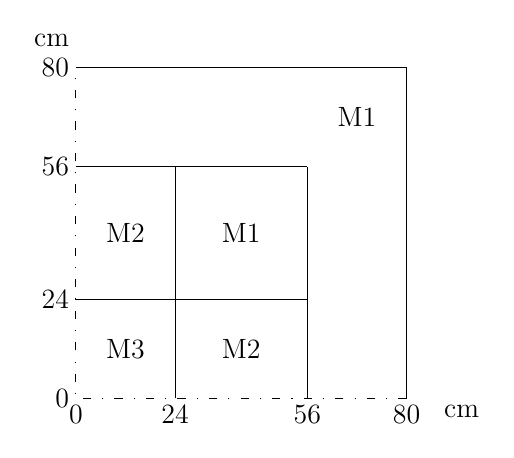
\begin{tikzpicture}[scale=0.7, transform shape]
\def\lenscale{0.075}
\def\x#1{#1*\lenscale}

\draw [loosely dashdotted] (\x{80},0) -- (0,0) -- (0,\x{80});

\draw (\x{24},0) -- (\x{24},\x{56});
\draw (0,\x{24}) -- (\x{56},\x{24});
\draw (\x{56},0) -- (\x{56},\x{56});
\draw (0,\x{56}) -- (\x{56},\x{56});
\draw (\x{80},0) -- (\x{80},\x{80});
\draw (0,\x{80}) -- (\x{80},\x{80});

\node at (\x{12},\x{12}) {\Large M3};
\node at (\x{40},\x{12}) {\Large M2};
\node at (\x{12},\x{40}) {\Large M2};
\node at (\x{40},\x{40}) {\Large M1};
\node at (\x{68},\x{68}) {\Large M1};

\foreach \xp in {0, 24, 56,80}
{
\node [below] at (\x{\xp},0) {\Large \xp};
\node [left] at (0,\x{\xp}) {\Large \xp};
}

\node [below] at (\x{80}+1,0) {\Large cm};
\node [left] at (0, \x{80}+0.5) {\Large cm};

\end{tikzpicture}
\caption{\label{fig:result.test.twigl}动态TWIGL二维基准题堆芯几何}
\end{figure}

\FloatBarrier
\subsection{动态LMW三维基准问题}

LMW(Langenbuch-Maurer-Werner)基准题\cite{langenbuch1977coarse,gehin1992quasi}是
三维两群扩散中子时空动力学基准题,
大小为$1/4$堆芯,几何尺寸110cm $\times$ 110cm $\times$ 200cm,
见\floatref{fig:result.test.lmw}。

\begin{figure}
\centering
\begin{subfigure}{.45\textwidth}
\hspace{-1.5cm}
\begin{tikzpicture}[scale=0.7, transform shape]
\def\lenscale{0.075}
\def\x#1{#1*\lenscale}

\draw [loosely dashdotted] (\x{110},0) -- (0,0) -- (0,\x{110});

\draw (\x{10},\x{0}) -- (\x{10},\x{10}) -- (\x{0},\x{10});
\draw (\x{50},\x{0}) -- (\x{50},\x{10}) -- (\x{70},\x{10}) -- (\x{70},\x{0});
\draw (\x{0},\x{50}) -- (\x{10},\x{50}) -- (\x{10},\x{70}) -- (\x{0},\x{70});
\node at (\x{30},\x{10}) {\Large M1};
\node at (\x{60},\x{5}) {\Large M2};
\node at (\x{5},\x{60}) {\Large M2};
\node at (\x{5},\x{5}) {\Large M2};

\draw (\x{30},\x{30}) rectangle (\x{50},\x{50});
\node at (\x{40},\x{40}) {\Large M2};

\draw (\x{70},\x{0}) -- (\x{70},\x{50}) -- (\x{50},\x{50})
      -- (\x{50},\x{70}) -- (\x{0},\x{70});
\node at (\x{60},\x{60}) {\Large M3};

\draw (\x{90},\x{0}) -- (\x{90},\x{70}) -- (\x{70},\x{70})
      -- (\x{70},\x{90}) -- (\x{0},\x{90});
\node at (\x{80},\x{80}) {\Large M4};

\draw (\x{110},\x{0}) -- (\x{110},\x{90}) -- (\x{90},\x{90})
      -- (\x{90},\x{110}) -- (\x{0},\x{110});

\foreach \xp in {0, 10,30,50,70,90,110}
{
\node [below] at (\x{\xp},0) {\Large \xp};
\node [left] at (0,\x{\xp}) {\Large \xp};
}

\node [below] at (\x{110}+1,0) {\Large cm};
\node [left] at (0, \x{110}+0.5) {\Large cm};

\draw [-latex new, arrow head=3mm] (-1.25,\x{50}) -- (\x{0},\x{60});
\draw [-latex new, arrow head=3mm] (-1.25,\x{50}) -- (\x{60},\x{10});
\node [left] at (-1.25,\x{50}) {\Large 第一组};

\draw [-latex new, arrow head=3mm] (-1.25,\x{20}) -- (\x{5},\x{10});
\draw [-latex new, arrow head=3mm] (-1.25,\x{20}) -- (\x{30},\x{40});
\node [left] at (-1.25,\x{20}) {\Large 第二组};

\end{tikzpicture}
\caption{横截面图}
\end{subfigure}
\\[1cm]
\begin{subfigure}{.45\textwidth}
\begin{tikzpicture}[scale=0.7, transform shape]
\def\lenscale{0.06}

\def\x#1{#1*\lenscale}
\def\zz#1{#1*\lenscale-0}
\def\z#1{#1*\lenscale}

\draw [very thick] (0,0) -- (\x{110},0) 
            -- (\x{110}, \zz{200}) -- (0, \zz{200});
\draw [loosely dashdotted] (0,0) -- (0, \zz{200});

\draw (0,\z{20}) -- (\x{90},\z{20}) -- (\x{90},\x{180}) -- (0,\zz{180});
\draw (\x{70},\x{20}) -- (\x{70},\x{180});

\node [left] at (0,0) {\Large 0};
\node [left] at (0,\z{20}) {\Large 20};
\node [left] at (0,\z{60}) {\Large 60};
\node [left] at (0,\z{100}) {\Large 100};
\node [left] at (0,\zz{180}) {\Large 180};
\node [left] at (0,\zz{200}) {\Large 200};

\node at (\x{30},\x{40}) {\Large M1};
\node at (\x{80},\x{100}) {\Large M3};
\node at (\x{100},\x{100}) {\Large M4};
\node at (\x{20},\x{190}) {\Large M4};
\node at (\x{40},\x{190}) {\Large M2};
\node at (\x{60},\x{190}) {\Large M2};
\draw [-latex new, arrow head=3mm] (-1,\x{190}) -- (\x{5},\x{190});
\node [left] at (-1,\x{190}) {\Large M2};

\draw [dashed] (\x{0},\x{100}) -- (\x{10},\x{100}) -- (\x{10},\x{200});
\draw (\x{10},\x{180}) -- (\x{10},\x{200});
\draw (\x{50},\x{200}) -- (\x{50},\x{100}) -- (\x{70},\x{100}) -- (\x{70},\x{200});
\draw [dashed] (\x{30},\x{180}) -- (\x{30},\x{200});

\node at (\x{60},\x{140}) {\Large M2};
\draw [-latex new, arrow head=3mm] (-1,\x{140}) -- (\x{5},\x{140});
\node [left] at (-1,\x{140}) {\Large M2};

\draw [-latex new, arrow head=3mm] (-1,\x{70}) -- (\x{5},\x{100});
\draw [-latex new, arrow head=3mm] (-1,\x{70}) -- (\x{60},\x{100});
\node [left] at (-1,\x{70}) {\Large 第一组};
\draw [-latex new, arrow head=3mm] (-1,\x{160}) -- (\x{5},\x{180});
\draw [-latex new, arrow head=3mm] (-1,\x{160}) -- (\x{40},\x{180});
\node [left] at (-1,\x{160}) {\Large 第二组};

\foreach \xp in {0,10,30,50,70,90,110}
{
\node [above] at (\x{\xp},\zz{200}) {\Large \xp};
}

\node at (-0.75,\zz{200}+0.75) {\Large cm};
\end{tikzpicture}
\caption{纵截面图(初始时控制棒位置)}
\end{subfigure}
\begin{subfigure}{.45\textwidth}
\begin{tikzpicture}[scale=0.7, transform shape]
\def\lenscale{0.06}

\def\x#1{#1*\lenscale}
\def\zz#1{#1*\lenscale-0}
\def\z#1{#1*\lenscale}

\draw [very thick] (0,0) -- (\x{110},0) 
            -- (\x{110}, \zz{200}) -- (0, \zz{200});
\draw [loosely dashdotted] (0,0) -- (0, \zz{200});

\draw (0,\z{20}) -- (\x{90},\z{20}) -- (\x{90},\x{180}) -- (0,\zz{180});
\draw (\x{70},\x{20}) -- (\x{70},\x{180});

\node [left] at (0,0) {\Large 0};
\node [left] at (0,\z{20}) {\Large 20};
\node [left] at (0,\z{60}) {\Large 60};
\node [left] at (0,\z{100}) {\Large 100};
\node [left] at (0,\zz{180}) {\Large 180};
\node [left] at (0,\zz{200}) {\Large 200};

\node at (\x{30},\x{40}) {\Large M1};
\node at (\x{80},\x{100}) {\Large M3};
\node at (\x{100},\x{100}) {\Large M4};
\node at (\x{20},\x{190}) {\Large M4};
\node at (\x{40},\x{190}) {\Large M2};
\node at (\x{60},\x{190}) {\Large M2};
\draw [-latex new, arrow head=3mm] (-1,\x{190}) -- (\x{5},\x{190});
\node [left] at (-1,\x{190}) {\Large M2};

\draw (\x{0},\x{60}) -- (\x{10},\x{60}) -- (\x{10},\x{200});
\draw [dashed] (\x{30},\x{200}) -- (\x{30},\x{60}) -- (\x{50},\x{60}) -- (\x{50},\x{200});
\draw (\x{50},\x{180}) -- (\x{50},\x{200});
\draw (\x{70},\x{180}) -- (\x{70},\x{200});

\draw [-latex new, arrow head=3mm] (-1,\x{30}) -- (\x{5},\x{60});
\draw [-latex new, arrow head=3mm] (-1,\x{30}) -- (\x{40},\x{60});
\node [left] at (-1,\x{30}) {\Large 第二组};
\draw [-latex new, arrow head=3mm] (-1,\x{160}) -- (\x{5},\x{180});
\draw [-latex new, arrow head=3mm] (-1,\x{160}) -- (\x{60},\x{180});
\node [left] at (-1,\x{160}) {\Large 第一组};

\node at (\x{40},\x{120}) {\Large M2};
\draw [-latex new, arrow head=3mm] (-1,\x{120}) -- (\x{5},\x{120});
\node [left] at (-1,\x{120}) {\Large M2};

\foreach \xp in {0,10,30,50,70,90,110}
{
\node [above] at (\x{\xp},\zz{200}) {\Large \xp};
}

\node at (-0.75,\zz{200}+0.75) {\Large cm};
\end{tikzpicture}
\caption{纵截面图(最终控制棒位置)}
\end{subfigure}
\caption{\label{fig:result.test.lmw}动态LMW三维基准题堆芯几何}
\end{figure}

\begin{table}
\centering
\caption{\label{tab:result.test.lmw.mat}动态LMW三维基准题材料截面}
\begin{tabular}{cccccc}
\toprule
材料 & 能群$g$ & $D_g/\mathrm{cm}$ & $\Sigma_{a,g}/\mathrm{cm}^{-1}$
    & $\nu\Sigma_{f,g}/n,\mathrm{cm}^{-1}$
    & $\Sigma_{s,1\rightarrow2}/\mathrm{cm}^{-1}$\\
\midrule
\multirow{2}{*}{M1} 
  & 1 & 1.423913 & 0.01040206 & 0.006477691 & \multirow{2}{*}{0.0175555} \\
  & 2 & 0.356306 & 0.08766217 & 0.1127328 &\\
\multirow{2}{*}{M2} 
  & 1 & 1.423913 & 0.01095206 & 0.006477691 & \multirow{2}{*}{0.0175555} \\
  & 2 & 0.356306 & 0.09146217 & 0.1127328 &\\
\multirow{2}{*}{M3} 
  & 1 & 1.425611 & 0.01099263 & 0.007503284 & \multirow{2}{*}{0.01717768} \\
  & 2 & 0.350574 & 0.09925634 & 0.1378004 &\\
\multirow{2}{*}{M4} 
  & 1 & 1.634227 & 0.002660573 & 0 & \multirow{2}{*}{0.02759693} \\
  & 2 & 0.264002 & 0.04936351 & 0 &\\
\bottomrule
\end{tabular}
\end{table}


算例包含两组控制棒,开始时第一组控制棒以3cm/s的速度拔出,
26.67s时停止。第二组控制棒从7.5s开始以同样的速度插入,47.5s时停止,
控制棒位置随时间变化见\floatref{fig:result.test.lmw.rob}。
\begin{figure}
\centering
\includegraphics[scale=0.9]{result-test-lmw-rob}
\caption{\label{fig:result.test.lmw.rob}LMW算例控制棒位置随时间变化图}
\end{figure}

裂变谱和缓发中子谱取$\chi_1=1$,$\chi_2=0$。
群速度为
\begin{align}
  \left\{
  \begin{aligned}
  v_1&=1.25\times10^7\mathrm{cm/s}\\
  v_2&=2.5\times10^5\mathrm{cm/s}
  \end{aligned}
  \right.
\end{align}
缓发中子有6组,见\floatref{tab:result.test.lmw.mat.c}。

\begin{table}
\centering
\caption{\label{tab:result.test.lmw.mat.c}动态LMW三维基准题缓发中子数据}
\begin{tabular}{ccc}
\toprule
缓发中子组 & 缓发中子份额$\beta_i$ & 衰变常数$\lambda_i/\mathrm{s}^{-1}$\\
\midrule
1 & 0.000247 & 0.0127\\
2 & 0.0013845 & 0.0317\\
3 & 0.001222 & 0.1150\\
4 & 0.0026455 & 0.3110\\
5 & 0.000832 & 1.400\\
6 & 0.000169 & 3.870\\
\bottomrule
\end{tabular}
\end{table}

\section{数值结果及验证}
\section{参数影响对比}
